
\documentclass[12pt]{iopart}
\usepackage[dvipsnames]{xcolor}
\usepackage{graphicx}
\usepackage{amssymb}
\usepackage{float}
\usepackage{multirow}
\usepackage[export]{adjustbox}
\usepackage[pagewise,modulo]{lineno}
\linenumbers
\newcommand{\gguide}{{\it Preparing graphics for IOP journals}}
\renewcommand{\ms}{\ensuremath{\mathrm{s}}}
\newcommand{\mi}{\ensuremath{\mathrm{i}}}
\newcommand{\BB}[1]{\textcolor{violet}{\emph{BB:} #1}}
%Uncomment next line if AMS fonts required
%\usepackage{iopams}  
\begin{document}

\title[]{A high-speed noise-free optical quantum memory}

\author{K.~T.~Kaczmarek$^{1,*}$, P.~M.~Ledingham$^1$, B.~Brecht$^1$, S.~E.~Thomas$^{1,2}$, G.~S.~Thekkadath$^3$, O.~Lazo-Arjona$^1$, J.~H.~D.~Munns$^{1,2}$, E.~Poem$^{1,4}$, A.~Feizpour$^1$, D.~J.~Saunders$^1$, J.~Nunn$^1$, I.~A.~Walmsley$^1$}
\address{$^1$Clarendon Laboratory, University of Oxford, Parks Road, Oxford, OX1 3PU, UK.\\
$^2$QOLS, Blackett Laboratory, Imperial College London, London SW7 2BW, UK. \\
$^3$University of Ottawa, 25 Templeton St, Ottawa, K1N 6N5, Canada.\\
$^4$Department of Physics of Complex Systems, Weizmann Institute of Science, Rehovot 7610001, Israel.}
\ead{$^*$k.kaczmarek1@physics.ox.ac.uk}

\maketitle

\textbf{Light is an ideal information carrier for quantum networks \cite{Kimble2008}: its quantum properties are not degraded by noise in ambient conditions and it has a large information capacity owing to its high bandwidth. The realisation of scalable high-speed photonic quantum networks, e.g. for quantum simulation and information processing, requires noise-free, low-latency, and technically simple quantum optical memories to overcome the exponentially poor scaling of current approaches based on linear optics. While low noise \cite{Chaneliere2005,Zhou2012,Maxwell2013,Ding2016,Distante2017,Seri2017}, high speed \cite{England2015}, and operation in ambient conditions \cite{Julsgaard2004,Hosseini2011,Ripka2016,Sibalic2016} have been shown separately, to date no atomic system satisfies all these desiderata simultaneously. Here we introduce the off-resonant cascaded absorption (ORCA) memory, and demonstrate for the first time the storage and recall of GHz-bandwidth single photons with zero added noise in a warm caesium vapour. Because of its technical simplicity, its high speed and its low noise, ORCA provides a viable route towards next generation, low-latency quantum-network technologies.}


The basic operating principle of a quantum optical memory is to prepare an empty storage state $|s\rangle$ and then map on-demand a quantum state of light to and from an atomic coherence between the ground state $|g\rangle$ and $|s\rangle$. With an additional intermediate atomic level $|e\rangle$ and an auxiliary control field this can be achieved - the input ``signal'' field drives the ``populated transition'' $(|g\rangle \leftrightarrow |e\rangle)$, while the control field drives the ``empty transition'' $(|e\rangle \leftrightarrow |s\rangle)$, as shown in Fig. \ref{fig:figFig1}. By using atomic ensembles, one increases the probability of a photon interacting with an atom, leading to strong light-matter coupling \cite{Thomas2016}. Traditionally the energy levels are arranged in a $\Lambda$ configuration: two ground states coupled via an excited state, since the long ground state coherence time gives prospects for long-distance quantum communication applications \cite{Bussieres2013}. Narrowband ($\sim$MHz), resonant $\Lambda$-type quantum optical memories based on electromagnetically-induced transparency (EIT) \cite{Chaneliere2005,Eisaman2005}, gradient echo memory (GEM) \cite{Hosseini2011} and the full atomic frequency comb (AFC) \cite{Jobez2015} protocol have performed well, with high efficiency \cite{Hedges2010} and preservation of photon statistics \cite{Seri2017} being demonstrated. However, their experimentally accessible narrow bandwidths combined with the additional need for preparation of the storage state (by means of optical pumping or spectral holeburning) limits their maximum clock-rate. Focussing on the requirements of local quantum networks, being able to operate at a high clock-rate for elementary building block synchronisation motivates the need for a broadband memory for short pulses of light \cite{Nunn2013}.

The $\Lambda$ configuration does allow the freedom of having the signal and control fields far-off single-photon resonance while remaining in two-photon resonance, as in the Raman memory scheme \cite{Reim2010a,Chrapkiewicz2017}. In this protocol, the control creates a broadband ``virtual'' resonance that the signal couples to. Because the signal is far detuned from the ``real'' atomic resonance, there is very little linear absorption. Interestingly, this means the system can be reduced to a beamsplitter-like interaction between different travelling optical modes and a stationary matter mode, where the ``reflectivity'' of the beamsplitter is determined by the storage and recall efficiencies \cite{Reim2012,Campbell2014,Fisher2016}. The caveat is that, in the absence of atomic selection rules, the control can off-resonantly couple to the populated transition, inducing spontaneous Raman scattering and polluting the storage state with spurious atomic excitations \cite{Michelberger2015}. The latter leads to four-wave mixing (FWM) noise in the same optical mode as the desired quantum signal when the memory is read out, deteriorating its photon statistics \cite{England2015,Michelberger2015}. Noise contamination of the signal, due to control field induced fluorescence or especially FWM in off-resonant broadband memories, remains one of the greatest challenges prohibiting network ready quantum memories.

\begin{figure}[h!]
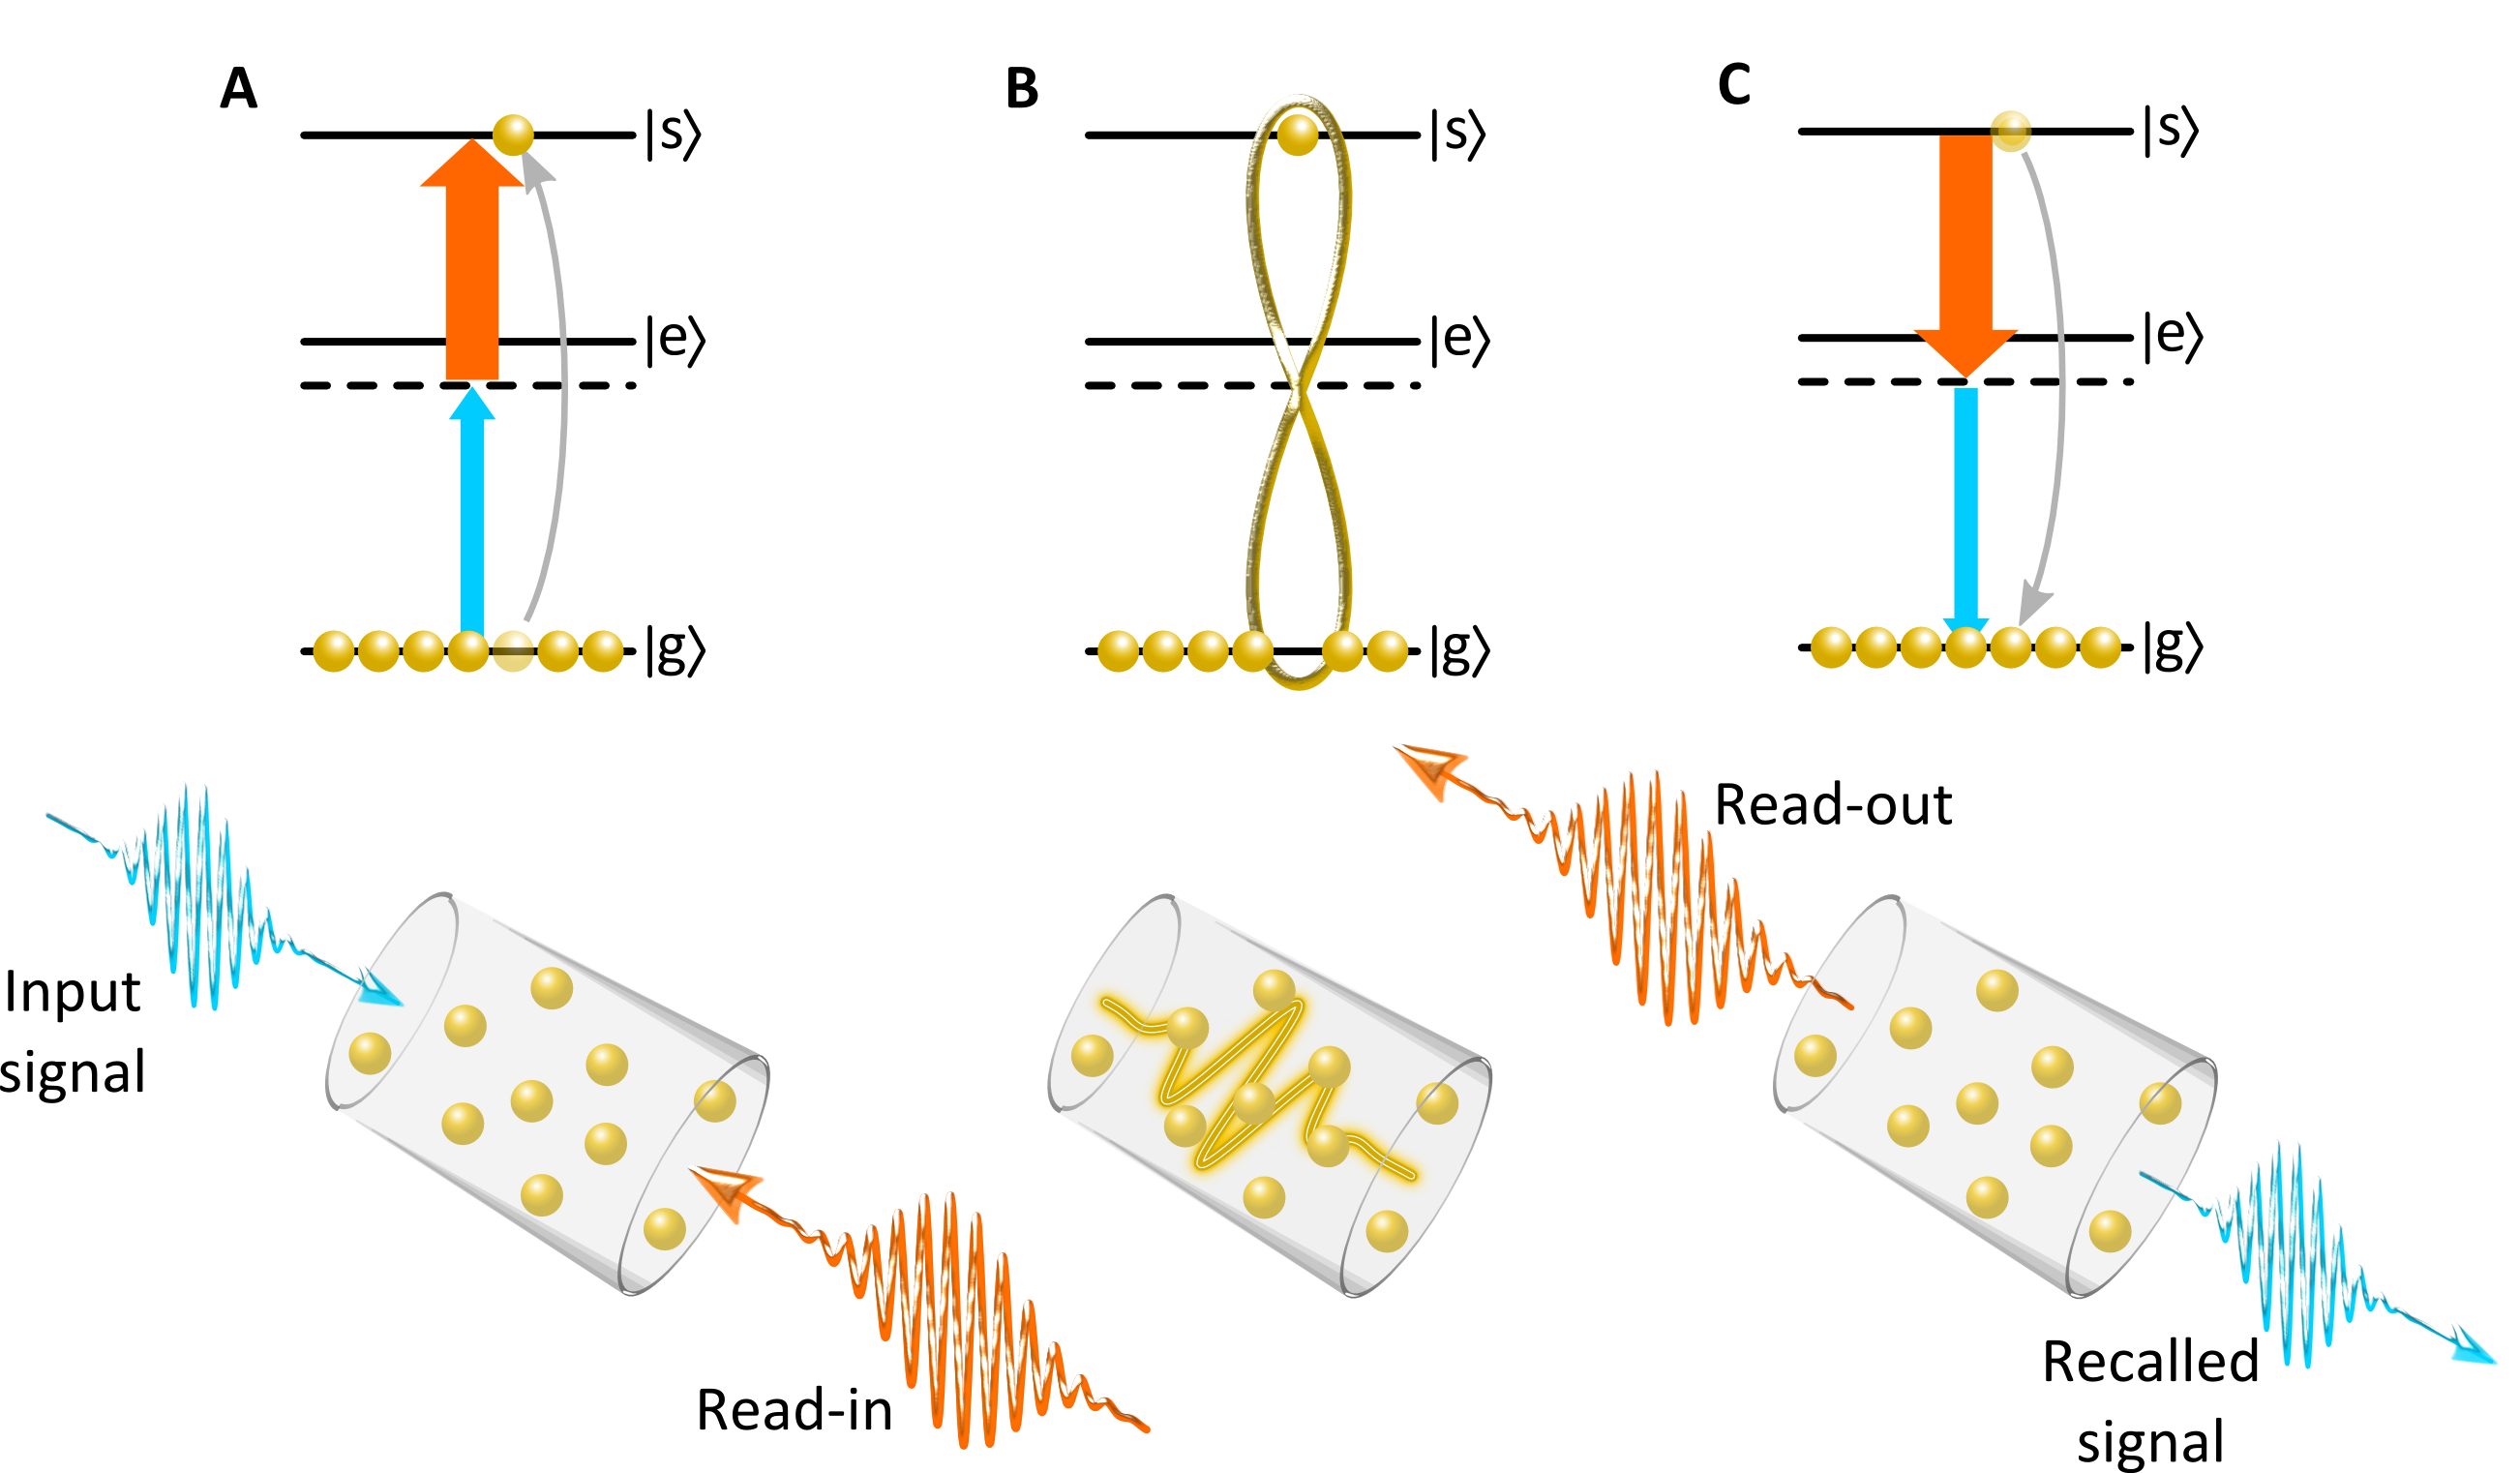
\includegraphics[width=\textwidth, right]{ORCApaperfig1.png} % this command will be ignored
\caption{\textbf{The ORCA protocol.}\newline  \textbf{a,} Storage: a weak ``signal'' field (blue) and strong ``control'' (orange) are overlapped counter-propagating in an atomic vapour. The broadband fields are on two-photon resonance with a doubly-excited storage state $|s\rangle$, while remaining far-detuned from the intermediate state $|e\rangle$.
\textbf{b,} The storage process maps the signal field to an atomic coherence (dashed line) between the ground $|g\rangle$ and storage $|s\rangle$ states. Motion-induced dephasing of the coherence is reduced owing to the counter-propagating field configuration.
\textbf{c,} Recall: re-applying the control pulse after the desired storage time leads to re-mapping of the atomic coherence back into an optical field and thus re-emission of the signal in the forward direction.
}\label{fig:figFig1}
\end{figure}

Here we introduce a new quantum memory scheme based on off-resonant cascaded absorption (ORCA) in a three-level ladder configuration that is optimised for warm atomic vapours (see Fig. \ref{fig:figFig1}). The operational principle is similar to the Raman memory: two broadband optical fields, signal and control, satisfy a two-photon resonance condition with a storage state, while individually being far-off resonance from their respective single-photon transitions. Unlike in $\Lambda$-type protocols, the ORCA memory bandwidth is not in principle limited by the ground state splitting, and the counter-propagating beam geometry reduces motional-induced dephasing of the stored coherence (see Supplementary Information), giving the potential for functional time-bandwidth products, i.e. the number of clock-cycles over which a memory allows synchronisation \cite{Finkelstein2017}.

In the new scheme, the storage state is a doubly-excited electronic state, which has no thermal excitations even at high temperatures. Therefore the protocol in principle requires no preparation of the atomic ensemble prior to storage, and there is no contamination of the recalled fields due to imperfect optical pumping. This points to the major benefit of ORCA storage in that it is {\it noise-free}. The signal and control wavelengths can be chosen such that the control photons are significantly detuned from the populated transition (THz detunings are readily available in the rich atomic structure of alkalis). This effectively eliminates any control field induced fluorescence noise. More importantly though, due to the ladder configuration, there is no scattering process that could populate the storage state, and so four-wave mixing noise is eliminated. Finally, efficient suppression of control field leakage on the output detection is readily achievable using off-the-shelf low-loss interference filters, and bolstered by the counter-propagating field configuration, in principle enabling \emph{end-to-end} device efficiencies approaching the \emph{internal} memory efficiency. The ORCA scheme is therefore a broadband and noise-free quantum optical memory protocol operating within a technically simple, room-temperature platform.

As a proof-of-principle demonstration, we implement the protocol with near-infrared light in warm caesium vapour (see Methods section for more details). We interface the ORCA memory with a 1 GHz bandwidth heralded single-photon source based on parametric down-conversion (PDC) \cite{Michelberger2015}, as shown in Fig. \ref{fig:figFig2}. In type-II PDC, a ``pump'' field is converted into orthogonally polarised pairs of photons by means of spontaneous scattering. In the weakly-pumped regime, when the pair production rate is low, the detection of a photon in one of the modes (``idler'') heralds the presence of another (``signal''), which we attempt to store.  We choose a storage time of 3.5 ns, as residual motion-induced dephasing limits the memory lifetime in the current implementation in Cs vapour to 5.4 ns (see Supplementary Information). Owing to the short lifetime, and without the need for time-consuming atomic state preparation, we are able to operate the experiment at the full 80~MHz repetition rate of our pump, as shown in Fig. \ref{fig:figFig3}a.

\begin{figure}[h!]
\centering
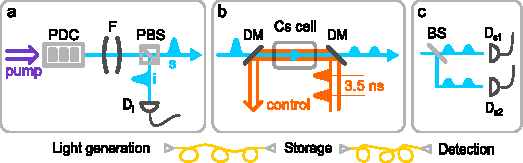
\includegraphics[width=0.83\textwidth, right]{Fig2SET2.pdf}
\caption{\textbf{Experimental setup.} \textbf{a,} Photon pairs at 852 nm are generated in parametric down-conversion (PDC) and consecutively filtered (F) to $\sim1$ GHz bandwidth. The signal (s) and idler (i) photons are separated on a polarizing beam splitter (PBS). While the idler photons are detected with a single-photon detector ($\mathrm{D_i}$), the signal photons are sent to the memory. \textbf{b, } Dichroic mirrors (DM) are used to combine the signal field with a bright, counter-propagating control field at 917 nm (read-in and read-out) inside a caesium vapour cell. After the memory, the transmitted and recalled light is sent to the detection stage. \textbf{c, } At the detection stage, the signal photons are split on a balanced beam splitter (BS) and detected by two single-photon detectors ($\mathrm{D_{s1}}$ and $\mathrm{D_{s2}}$) in a Hanbury-Brown-Twiss configuration.}
\label{fig:figFig2}
\end{figure}

Fig. \ref{fig:figFig3}a shows a section of the photon arrival time trace with the control field off (``SIG'') and on (``MEM''). We measure a memory efficiency (storage and recall) of $\eta=14.6\pm1.9\;\%$. Higher efficiencies can be reached by stronger driving, increased atomic density, and appropriate shaping of the control pulse, as predicted by existing theory of quantum memories based on three-level systems \cite{Nunn2007,Novikova2007,Gorshkov2007}. Due to the absence of four-wave mixing gain \cite{Thomas2016} however, ORCA is in principle capable of reaching these high efficiencies without adding noise.

We benchmark the noise performance of the memory by evaluating $\mu_1=\langle n^\mathrm{noise}\rangle/\eta$, i.e. the ratio of the average number of noise photons per control pulse $\langle n^\mathrm{noise}\rangle$ and $\eta$ \cite{Gundogan2015}. We find $\mu_1\leq(39.4\pm0.2)\times10^{-6}$, the lowest ever reported from an atom-based quantum memory. Note that the measured $\mu_1$ is an upper bound, limited by the technical noise (dark counts) of our detectors.

To verify the quantum performance of the memory we measure the photon number statistics and correlations of the recalled signal, and compare it with the input. Fig. \ref{fig:figFig3}b shows the detected coincidence clicks between the detectors $\mathrm{D_{i}}$ \& $\mathrm{D_{s1/2}}$ at different times with the control off (``SIG'') and on (``MEM''). First, we evaluate the cross-correlation function $g^{(1,1)}$ of signal and idler photons (see Methods section). Values of $g^{(1,1)}>2$ signify non-classical correlations \cite{Farrera2016}. We measure $g^{(1,1)}=131.3\pm0.2$ for the input signal field, and upon recall obtain $g^{(1,1)}=120.0\pm0.1$, clearly exceeding the classical bound and demonstrating the preservation of non-classical correlations in ORCA. We attribute the reduction of the $g^{(1,1)}$ in the read-out to dark count contamination.

\begin{figure}[h!]
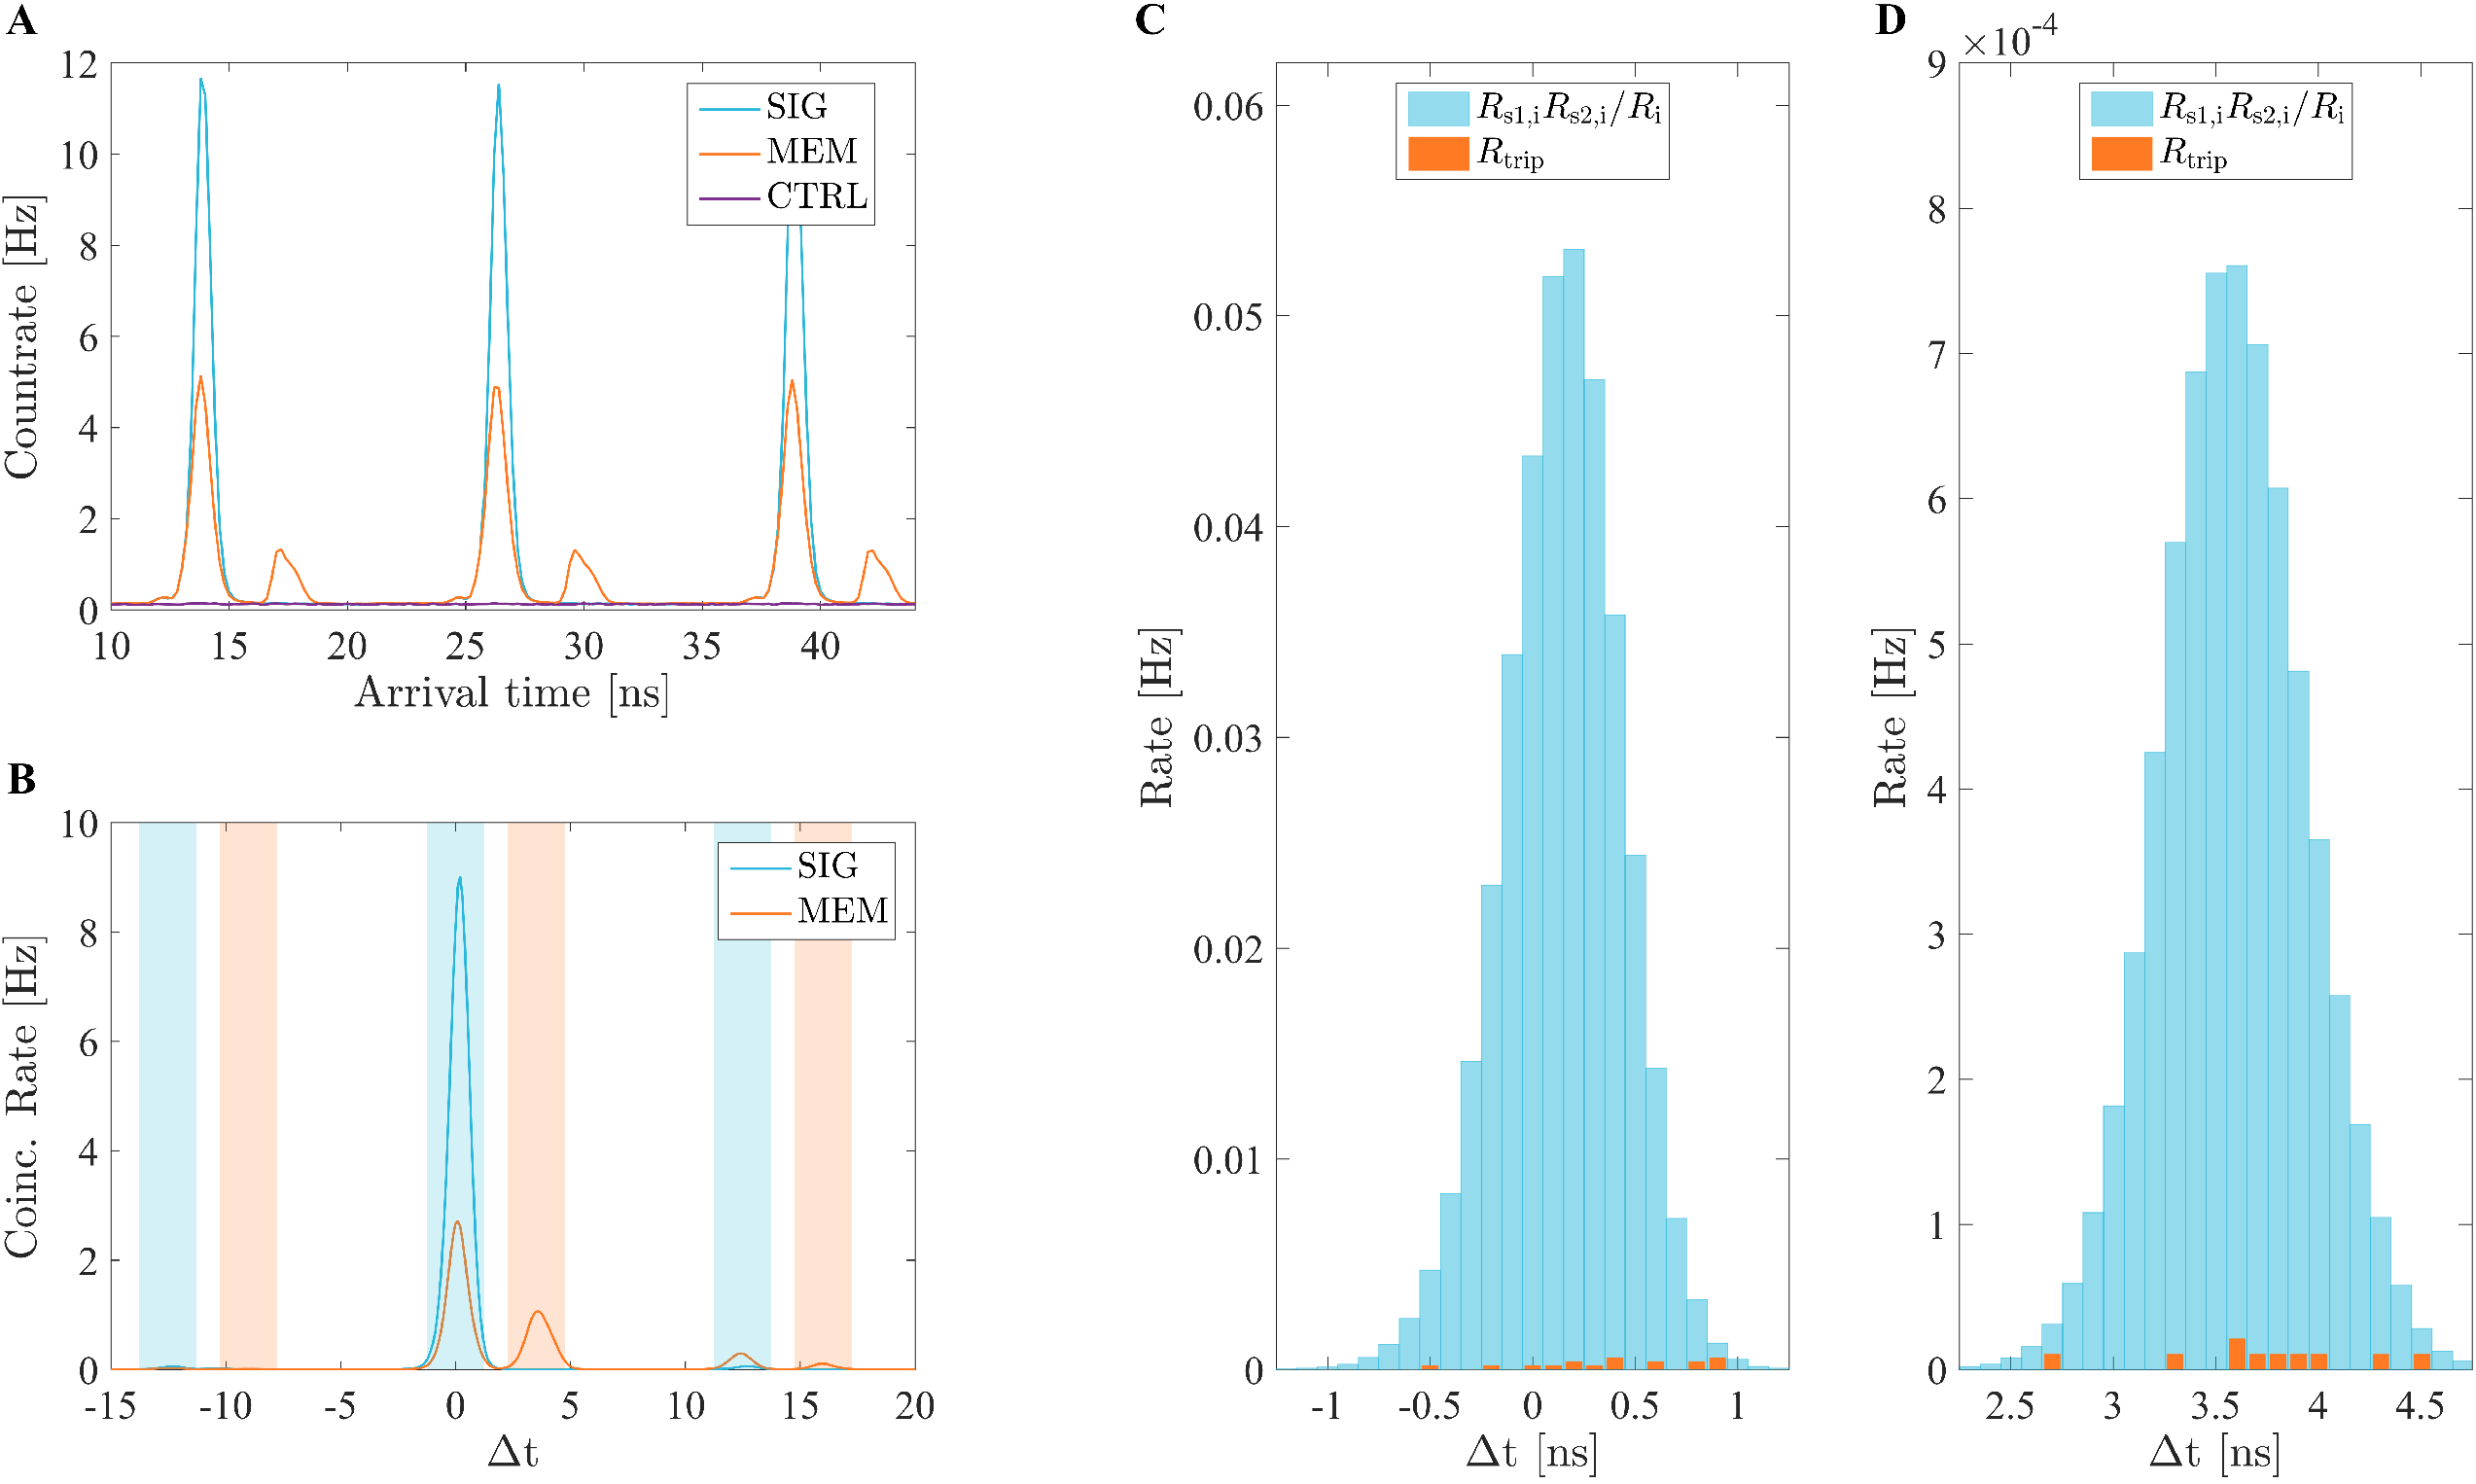
\includegraphics[width=\textwidth, right]{ORCApaperFig3c.pdf} 
\caption{\textbf{Storage of single photons using ORCA.}\newline \textbf{a,} Histogram showing timing of total signal detector clicks with respect to external 1 MHz trigger. ``SIG'' is the signal field with the control field off, ``MEM'' is the signal field with the control on for a storage time of 3.5 ns. ``CTRL'' has the control field on, but with no input signal. Any photons detected in the ``CTRL'' configuration correspond to noise generated in the memory. \textbf{b,} Histogram of the time difference $\Delta t$ between idler and total signal detector clicks, with the control off (``SIG'') and on (``MEM''). The blue (orange) shaded areas correspond to the integration windows for the SIG (MEM) setting. The peaks at 12.5 and 16 ns in the ``MEM'' trace come from consecutive control pulses reading out residual coherence (see Supplementary Information). \textbf{c,} Input signal: orange - histogram of the time difference $\Delta t$ between idler detector clicks, and signal detector coincidences, i.e. triple coincidence histogram $R_\mathrm{trip}$; blue - product of the two-fold coincidences between the idler and two signal detectors, $R_\mathrm{s1,i}$ and $R_\mathrm{s2,i}$, normalized by the idler counts $R_\mathrm{i}$, i.e. predicted triple coincidence histogram for coherent light of the same average photon rate as the PDC. The ratio between the two histograms corresponds to the measured heralded auto-correlation function $g^{(2)}_\mathrm{h}$. \textbf{d,} Same as \textbf{c}, but for the recalled signal.}
\label{fig:figFig3}
\end{figure}


In order to determine whether ORCA preserves the quantum statistics of the input, we next evaluate the second-order heralded auto-correlation function $g^{(2)}_\mathrm{h}$ (see Methods section). A value of $g^{(2)}_\mathrm{h}<1$ is a direct measure of quantum statistics, with $g^{(2)}_\mathrm{h}=0$ corresponding to a perfect single photon \cite{Zhou2012}. We measure the $g_\mathrm{h}^{(2)}$ of our input signal (Fig. \ref{fig:figFig3}c) to be $0.020\pm0.005$, as expected from a weakly pumped PDC source \cite{Michelberger2015}. Upon recall (Fig. \ref{fig:figFig3}d), we obtain $g_\mathrm{h}^{(2)}=0.028\pm0.009$, the lowest ever measured from a room-temperature quantum memory. The agreement between input and output $g_\mathrm{h}^{(2)}$ provides further strong experimental confirmation that the atomic memory adds zero noise, similarly to a non-atomic memory based on electronically switched free-space cavities \cite{Kaneda2015}.

In conclusion, we have demonstrated the first noise-free broadband atomic quantum memory protocol at room temperature, based on off-resonant cascaded absorption (ORCA), successfully storing and recalling a single photon from a warm vapour containing $\sim10^{10}$ moving atoms interacting with $\sim10^{9}$ control photons.

In the current experiment in Cs we achieved a time-bandwidth product of $\sim5$. By using a different atomic species with smaller signal/control wavelength mismatch, the memory lifetime can be significantly extended. Recently, Finkelstein et al. \cite{Finkelstein2017} demonstrated a fast ladder memory (FLAME) —-- equivalent to ORCA when far-detuned —-- with classical signal pulses in rubidium vapour. Here, the near-degeneracy of the signal and control fields allowed close to Doppler-free operation, with a memory lifetime $\sim85$ ns, granting Finkelstein et al. a time-bandwidth product of $\sim50$.

With foreseeable improvements in memory efficiency and lifetime, ORCA will be capable of achieving the performance necessary for high clock-rate synchronisation of probabilistic operations in local quantum networks \cite{Nunn2013}. Furthermore, ORCA is compatible with waveguide structures \cite{Sprague2014,Kaczmarek2015}, enabling efficient interfacing with integrated optical circuits \cite{Harris2017}. This will facilitate the creation of photonic quantum states of unprecedented scale, opening the way to a new regime of quantum simulation, computation and sensing.

\section*{Methods}
\subsection*{Experiment}
We use the Cs D2 line at 852 nm for our signal field, with $6S_{1/2}(F=4)$ as the ground state $|g\rangle$ and the $6P_{3/2}(F=3,4,5)$ manifold as the ORCA intermediate state $|e\rangle$. A strong 917 nm control field couples this signal to the storage state $|s\rangle$, i.e. the $6D_{5/2}(F=2,3,4,5,6)$ manifold. This configuration can be reasonably treated as a three-level system under broadband excitation \cite{Huber2011}. We detune both fields by 6 GHz from the intermediate state towards the ground state, enabling good coupling with negligible ($<2\%$) linear absorption.

The generation of heralded single photons is achieved using type-II parametric down-conversion (PDC) in a periodically poled potassium titanyl phosphate waveguide. The source generates THz-bandwidth pairs of signal and idler photons, both of which are consequently filtered down to $\sim1$ GHz bandwidth centred at the signal frequency using a series of Fabry-Per\'ot etalons and grating filters \cite{Michelberger2015}. We send the PDC idler to a single-photon silicon avalanche photodiode (APD) and the signal towards the memory. Our heralding efficiency before the memory is $\eta_\textrm{herald}\approx5\,\%$. The source is pumped at a rate of 80 MHz from a frequency doubled actively mode-locked titanium sapphire laser, with a $\sim0.8\%$ chance of producing a photon pair of the correct bandwidth per pump pulse.

The control field is derived from a second mode-locked titanium sapphire laser, locked-to-clock with the PDC pump. The laser bandwidth is $\sim0.9$ GHz, corresponding to a pulse duration of $\sim500$ ps. In order to investigate storage times $<12.5$ ns, i.e. smaller than the time between consecutive pulses from the laser, we use an unbalanced Mach-Zehnder interferometer with a variable delay in one arm to split the control pulse train into two: read-in and read-out, and delay them with respect to each other. The read-in and read-out control pulse energies are 0.21(1) and 0.97(1) nJ, respectively.

We combine the signal and counter-propagating control fields on a dichroic mirror. Both beams are focused down to a $\sim300\;\mu$m waist and temporally overlapped inside a 72 mm -long uncoated glass Cs-133 vapour cell heated to $\sim 91^o$C.

After the signal field leaves the memory it is sent into a Hanbury-Brown-Twiss detection setup, composed of a balanced beamsplitter and two fibre-coupled single-photon silicon APDs connected to a time-to-digital converter (same as the idler detector), allowing us to reconstruct the quantum photon number statistics of the stored/recalled signal fields.

\subsection*{Photon statistics}
By evaluating the $g^{(1,1)}$ cross-correlation function between the signal and idler (herald) pulses, we obtain a measure for the strength of the correlations between them. $g^{(1,1)}$ is defined as $p_\mathrm{si}/p_\mathrm{s}p_\mathrm{i}$, where $p_\mathrm{si}$ is the probability for a signal-idler coincidence click, and $p_\mathrm{s(i)}$ is the signal (idler) click probability. Values of $g^{(1,1)}>2$ signify non-classical correlations. To calculate $g^{(1,1)}$ from the measurements, we use

\begin{equation}
g^{(1,1)}=\frac{R_\mathrm{s,i}}{R_\mathrm{s}R_\mathrm{i}}R_\mathrm{T},
\end{equation}
where $R_\mathrm{s,i}$ is the sum of $\mathrm{D_{i}}$-$\mathrm{D_{s1}}$ and $\mathrm{D_{i}}$-$\mathrm{D_{s2}}$ coincidences, $R_\mathrm{T}$  is the total number of trigger events during the whole measurement time, $R_\mathrm{s}$ is the sum of $\mathrm{D_{s1}}$ and $\mathrm{D_{s2}}$ clicks, and $R_\mathrm{i}$ is the number of $\mathrm{D_{i}}$ clicks.

The heralded auto-correlation is defined as $g^{(2)}_\mathrm{h}=p_\mathrm{(s1,s2|i)}/p_\mathrm{(s1|i)}p_\mathrm{(s2|i)}$. Here, $p_\mathrm{(s1,s2|i)}$ is the conditional probability of detecting a coincidence between $\mathrm{D_{s1}}$ and $\mathrm{D_{s2}}$ given a click in $\mathrm{D_{i}}$, and $p_\mathrm{(s1|i)}$ ($p_\mathrm{(s2|i)}$) is the probability to detect a click in $\mathrm{D_{s1}}$ ($\mathrm{D_{s2}}$) given a click in $\mathrm{D_{i}}$. Any $g^{(2)}_\mathrm{h}<1$ verifies non-classical photon-number statistics. We evaluate $g^{(2)}_\mathrm{h}$ using

\begin{equation}
g^{(2)}_\mathrm{h}=\frac{R_\mathrm{trip}}{R_\mathrm{s1,i}R_\mathrm{s2,i}}R_\mathrm{i},
\end{equation}
where $R_\mathrm{trip}$ is the number of triple coincidences between $\mathrm{D_{i}}$, $\mathrm{D_{s1}}$, and $\mathrm{D_{s2}}$, $R_\mathrm{i}$ is the number of idler clicks, and $R_\mathrm{s1(2),i}$ is the number of $\mathrm{D_{i}}$-$\mathrm{D_{s1}}$ ($\mathrm{D_{i}}$-$\mathrm{D_{s2}}$) coincidences. More details can be found in the Supplementary Information.

\subsection*{Theoretical modeling}

An ab-initio model using Maxwell-Bloch equations is used to characterize the memory performance. We obtain equations for the time evolution of  velocity class ensembles $\hat{\rho}(v)$ coupled with signal and control fields. We consider 12 atomic states corresponding to the hyperfine levels of the $6S_{1/2}, 6P_{3/2}, 6D_{5/2}$ multiplets. The fields are coupled to the atomic states through a master equation with a Hamiltonian under electric dipole and rotating wave approximations, and in an appropriately chosen rotating frame, as well as Lindblad terms accounting for spontaneous decay5. The control field is taken to be strong enough to propagate without dispersion from the atomic vapour. The signal field is coupled to the total density matrix $\hat{\rho}=\int \mathrm{d}v g(v) \hat{\rho}(v)$ (where $g(v)$ is a Maxwell-Boltzmann velocity distribution) through the source term of a wave equation under the slowly-varying envelope approximation.

We numerically solve these equations using experimental parameters with only electric dipole matrix elements as free parameters. Once a good fit is found for the memory efficiencies as a function of control pulse power, the same parameters are used throughout this work.


%\include{Citations}

\section*{References}
\bibliographystyle{unsrt}
\bibliography{ladderPaper} 

\section*{Supplementary Information}
\setcounter{figure}{0}
\renewcommand{\thefigure}{S.\arabic{figure}}
\setcounter{table}{0}
\renewcommand{\thetable}{S.\arabic{table}}
\setcounter{subsection}{0}
\renewcommand{\thesubsection}{S.\arabic{subsection}}
\setcounter{equation}{0}
\renewcommand{\theequation}{S.\arabic{equation}}

\subsection{Memory lifetime \label{lifetime}}
There are three effects limiting the lifetime of this ORCA memory: spontaneous emission from the doubly excited atomic state, motion-induced dephasing due to the Doppler effect, and destructive interference between hyperfine components of the excited state.

Motion-induced dephasing arises due to the Doppler effect and atomic motion in a warm ensemble. This is because the stored excitation is spread over atoms belonging to different velocity classes in the ensemble. Due to the Doppler effect, each velocity class experiences the signal and control fields shifted in frequency. As a consequence, the phase of the stored coherence evolves at different rates in different velocity classes. The motion-induced dephasing lifetime is \cite{Zhao2009} $\tau_D = k_r v_s$, where $v_s = \sqrt{k_B T/m}$, and $k_r=\frac{2\pi}{\lambda_\mathrm{s}} -\frac{2\pi}{\lambda_\mathrm{c}}$; with $T$ the temperature of the atomic vapour, $m$ the mass of the atom, and $\lambda_\mathrm{s/c}$ the wavelengths of the signal and control fields. In other words, the collective coherence will dephase at a rate proportional to the square root of the temperature, and the wavenumber mismatch of the fields.

In the absence of optical pumping, the off-resonant two-photon excitation that stores the signal photon has contributions from all allowed paths connecting the $6S_{1/2}$ and $6D_{5/2}$ manifolds. The resulting excitation is spread across components of the $6D_{5/2}$ manifold. During storage time these components oscillate with different rates as given by their energy differences, and at read-out time they can interfere destructively in the creation of the read-out photon. Optical pumping restricting the memory interaction to the hyperfine levels $F=4 \rightarrow F=5 \rightarrow F=6$ reduces this effect.

\begin{figure}[h]
\centering
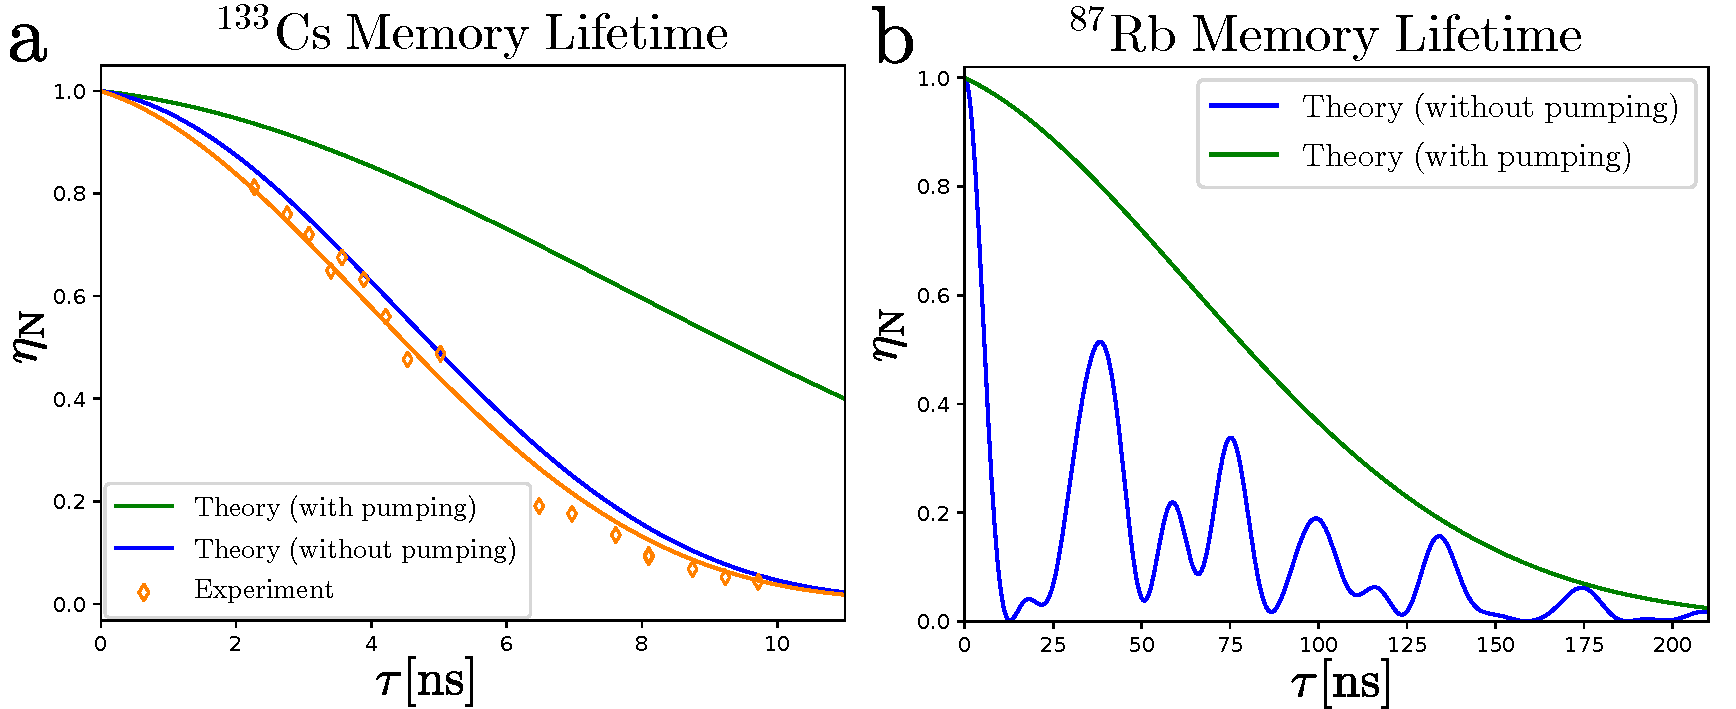
\includegraphics[width=\linewidth]{lifetime_cs_rb.pdf}
\caption{\textbf{a}. The measured (normalised to $\tau=0$) memory efficiency $\eta_\mathrm{N}$ (orange diamonds, experimental errors are smaller than the markers) versus storage time $\tau$ along with a theory fit of the memory lifetime curve (orange line) yielding a (1/e) lifetime of $5.5\pm0.1$ ns. Also shown is the predicted memory lifetime curves with (green) and without (blue line) optical pumping. \textbf{b}. Memory lifetimes predicted from theory for $^{87}\mathrm{Rb}$ with (green) and without (blue line) optical pumping.}
\label{fig:figLifetime}
\end{figure}

We determine the actual memory lifetime by measuring the memory efficiency for different storage times using a weak coherent state signal. In Fig. \ref{fig:figLifetime}a we show the measured normalized memory efficiency versus storage time (orange diamonds). Fitting our model to the data we obtain a $1/e$ lifetime of $5.5\pm 0.1$ ns. Using the Maxwell-Bloch model directly we predict a memory lifetime of 5.9 ns, very close to the measured one.

While seemingly short, the memory lifetime can be extended through optical pumping to reduce the destructive interference of hyperfine components or by using a different atomic species with a smaller signal/control wavenumber mismatch. If we choose the dipole couplings in the model such that only the transition $F=4 \rightarrow F=5 \rightarrow F=6$ is allowed (as with optical pumping), we obtain a memory lifetime of 11.5 ns (the green curve in figure \ref{fig:figLifetime}a). Furthermore, a simulation of the $5S_{1/2}\rightarrow5P_{3/2}\rightarrow5D_{5/2}$ cascade in $^{87}\mathrm{Rb}$ (signal at 780~nm, control at 776~nm) yields a memory lifetime of $99$~ns as shown by the green curve in \ref{fig:figLifetime}b.

\subsection{Experimental setup \label{setup}}

\begin{figure}[h!]
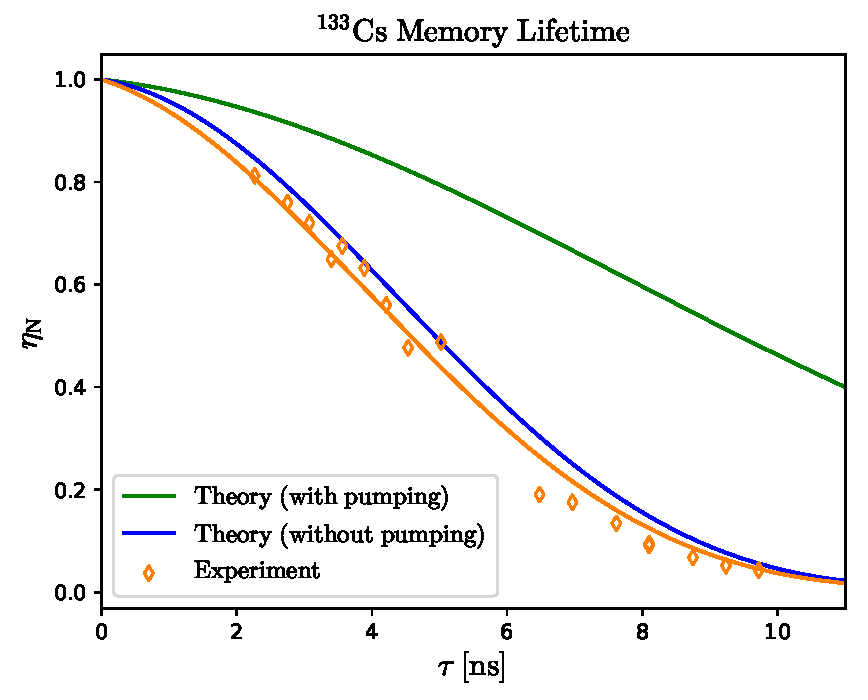
\includegraphics[width=\textwidth]{doppler_dephasing_cs3.pdf} % this command will be ignored
\caption{\textbf{Schematic of the experimental setup for ORCA}. \textbf{(a) }  Signal generation stage. \textbf{(b) } Control generation stage. \textbf{(c) } Memory and detection stage. SHG - periodically poled potassium titanyl (ppKTP) bulk crystal; ppKTPw - ppKTP waveguide; DM - dichroic mirror; FP - Fabry-P\'erot etalon; PBS - polarizing beamsplitter; HWP - half-wave plate; QWP - quarter-wave plate; APD - avalanche photodiode detector; BF - bandpass filter.}\label{fig:figSup1}
\end{figure}

Figure \ref{fig:figSup1} shows a schematic of the ORCA experimental setup. For the memory lifetime measurement (section \ref{lifetime}) we produce a weak coherent state signal (average photon number of $\sim2$) by picking pulses using a fast Pockels cell (extinction ~20,000:1) at a 1 MHz rate from a 80 MHz train of pulses generated by a $\sim330$ ps actively mode-locked titanium sapphire (Ti:Sapph) laser operated at 852 nm and filtered by a Fabry-P\'erot (FP) etalon down to 0.81 GHz bandwidth. Using a scanning FP etalon connected to a PC running LabVIEW, we reference-lock the Ti:Sapph's center frequency (via the voltage on a Gires-Tournois-Interferometer inside the laser cavity) to a continuous wave (CW) laser locked to the Cs D2 line via saturated absorption spectroscopy. 

We generate the control field from a second $\sim500$ ps actively mode-locked Ti:Sapph laser operated at 917 nm, with its center frequency locked using a wavelength meter, and its repetition rate locked to the signal Ti:Sapph using a commercial lock-to-clock (L2C) system. We use an unbalanced free-space Mach-Zehnder interferometer to split the 80 MHz pulse train into two, with a variable delay $<\sim4$ ns between them, in order to investigate storage times $<12.5$ ns. For storage times $6\;\mathrm{ns}<\tau<12.5$ ns we use the L2C electronics to change the timing between signal and control pulse trains such that read-in and read-out are switched. We also use the L2C to temporally overlap the signal and control pulses in the memory cell.

We combine the signal and control fields on a dichroic mirror, which - followed by a 10 nm bandpass filter centred at 850 nm - reduces control field leakage to the detectors from back-reflections by a factor of $\sim10^9$. We focus signal and control beams down to a $\sim300\;\mu$m waist inside a 72 mm -long uncoated caesium borosilicate reference cell heated using a custom-made oven. We estimate the cell temperature to be $\sim 91^o$C by frequency scanning a weak CW probe laser over the Cs D2 line and fitting a Voigt profile to the measured atomic absorption line.

After the signal field passes through the memory and the filters, we send it into a Hanbury-Brown-Twiss setup, composed of a half-waveplate, polarising beamsplitter and two fibre-coupled single-photon avalanche photodiodes. The two signal and the idler avalanche photodiodes were connected to a time-to-digital converter. For the weak coherent state data and cross-correlation measurements, we add the counts on the two signal detectors to estimate the total magnitude of the transmitted/recalled signal.

\subsection{Photon source and setup losses}
The generation of heralded single photons is achieved using type-II parametric down-conversion in a ppKTP waveguide. The waveguide, operated in a single-pass configuration and of length 20$\,$mm, is pumped with pulses of approximately 270 ps duration at a wavelength of 426\,nm. This pump light is derived by doubling the above mentioned 852\,nm Ti:Sapph laser via second harmonic generation in a separate 2$\,$mm long ppKTP crystal. With an incident average power near 700\,mW at 852\,nm at the crystal we arrive with 4\,mW average power at 426\,nm before the PDC waveguide. This light is then coupled to the waveguide with a total transmission of $<10\%$ including the loss at the in- and out-coupling lenses. We note that the waveguide is not single-mode for the pump wavelength and that the coupling is optimised to primarily excite the fundamental spatial mode, resulting in a low overall transmission. The generated frequency-degenerate but polarisation-orthogonal signal and idler modes have a bandwidth on the order of $1\,$THz. 

We characterise beam propagation transmission using an ``alignment'' mode, which is coupled to the fundamental mode of the waveguide, and thereby comparable to the signal and idler modes allowing for ``classical'' measurements to be made. These modes are then subject to frequency filtering. First, we apply coarse filtering using edge filters. Then, the modes are spatially separated via a PBS to then be coupled to their own single-mode fibre (SMF) with an efficiency of $(64 \pm 1)\%$ for the signal mode and $(53 \pm 2)\%$ for the idler mode. The modes are then out-coupled and recombined on a PBS forming a common spatial mode to then pass two etalons, one of FSR$\,$=$\,$18.4$\,$GHz and one of $103\,$GHz, which gives an effective FSR of $~1\,$THz (lowest common multiple). This is followed by a holographic volume Bragg grating with a width $\sim$100$\,$GHz. Using a narrowband ($\sim\,$MHz) probe the measured width this filtering has is $1\,$GHz for both modes. Finally the modes are separated spatially again via a PBS, the idler coupled to an APD (efficiency $\eta \approx 50\%$, dark counts = $163\pm 1\,$Hz) via a multimode fibre (total transmission from after waveguide to in front of idler detector is $\eta_\textrm{i,filt}\,=\,(9.7\pm0.1)\,\%$), while the signal is coupled to a SMF to be out-coupled and steered to the memory (total transmission from after waveguide to after this SMF is $\eta_\textrm{s,filt}\,=\,(12.8 \pm 0.3)\,\%$). 

The filtered signal photon is now steered toward the memory. First there is an edge filter which is used to prevent the 917$\,$nm control from backward-coupling toward the source which presents additional loss to the signal mode. Further, the caesium cell used is uncoated, adding more loss. After passing the cell, the signal mode is then separated from the control mode via a dichroic mirror and finally passes a bandpass filter about 852$\,$nm before entering a Hanbury-Brown-Twiss set-up. The mode is spatially separated into two and coupled to two APDs ($\eta\approx50\,\%$ dark counts = $296 \pm 2\,$Hz and $\eta\approx50\,\%$ dark counts = $356 \pm 2\,$Hz) via SMF. The total transmission from the source to in front of these detectors (averaging over the two SMF couplings) is $\eta_\textrm{s,total}\,=\,3.7\pm0.1\,\%$. That is to say, the photon undergoes an additional $\eta_\textrm{s,add}\,=\,30\,\%$ transmission from after the initial filtering stage.

For all results presented in this paper we operated with an average pump power of $4\,$mW in front of the waveguide in-coupling lens. Typically, we measure an idler (signal) count rate of around $30\,$kHz ($10\,$kHz) for the case of no control pulses. The typical Klyshko efficiency $\eta_k$ measured is $0.7\,\%$. This allows to calculate a heralding efficiency of $\eta_\textrm{herald} = \eta_k/\eta_{\textrm{det}}/\eta_\textrm{s,add} = 4.7\,\%$, which is well above the $\mu_1$ of the memory, as required for single-photon storage \cite{Gundogan2015}. Finally, the heralding efficiency just after the waveguide is $\eta_\textrm{s,waveguide} = \eta_k/\eta_{\textrm{det}}/\eta_\textrm{s,total} = 38\,\%$. The missing factor of $2.6$ we attribute to not measuring explicitly the loss inside the waveguide, the out-coupling loss from waveguide to free-space and the potential frequency mismatch of the etalon centroids between signal and idler.

\subsection{Data acquisition and post-processing}
During the measurements, the settings of three mechanical shutters which selectively blocked the read-in, read-out, and signal beams defined four different configurations (see Fig. \ref{fig:measurement_settings}): memory measurements with all three shutters open ("MEM"); read-in measurements with signal and read-in shutters open, and read-out shutter closed ("RI"); signal measurements with signal shutter open and both read-in and read-out closed ("SIG"); and noise measurements with read-in and read-out shutters open and signal shutter closed ("CTRL"). A single measurement consisted of recording the number of detector counts registered in a period of 180~s in the "MEM" configuration, followed by recording the total counts over 10~s in the "RI", "SIG", and "CTRL" configurations. After completion of all four configurations, the corresponding data was written to disk and the measurement repeated. This mode of operation was chosen in order to mitigate the effect of slow drifts in the setup that arose from changes in the laboratory temperature and humidity.

\begin{figure}[h!]
\centering
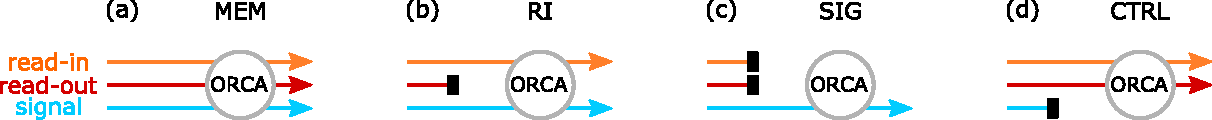
\includegraphics[width=\linewidth]{Sup1KTK.pdf}
\caption{\textbf{Schematic of the different measurement settings.} Black rectangles signify a closed shutter. For more information see the text.}
\label{fig:measurement_settings}
\end{figure}

For each configuration in each measurement, we recorded arrival time histograms for the three detectors ($\mathrm{D_{i}}$, $\mathrm{D_{s1}}$, $\mathrm{D_{s2}}$). These are histograms of firing times of the single-photon detectors with respect to a 1~MHz trigger signal derived from the Ti:Sapph recorded with the time-to-digital converter (TDC). We chose a time-bin width of 200~ps as a compromise between temporal resolution of the TDC and total number of time bins in the histogram. For data visualization, we added all arrival time histograms and normalised them to both the number of measurements (521) and the respective measurement duration (180~s for "MEM", 10~s else), obtaining a count rate per time bin in units of Hertz. 

Fig. \ref{fig:arrival_time_02} shows a section of the arrival time histograms. To reduce the impact of spurious noise counts (primarily from detector dark counts), we applied time gates to the recorded arrival time histograms and only kept events that lay within the time gates. The time gates for the read-in pulses (blue regions) are centred around the maxima of the individual read-in peaks and have a width of 2.5 ns, chosen such that the peaks were completely inside the gating region. Similar time gates were chosen for the recalled light, where the centre of these read-out gates (orange regions) was offset from the corresponding read-in time gates by 3.5 ns, which was the storage time chosen for the experiment. By integrating the detection events over only the gate regions, we calculated the read-in, read-out, and total memory efficiencies stated in the main text.  

\begin{figure}
\centering
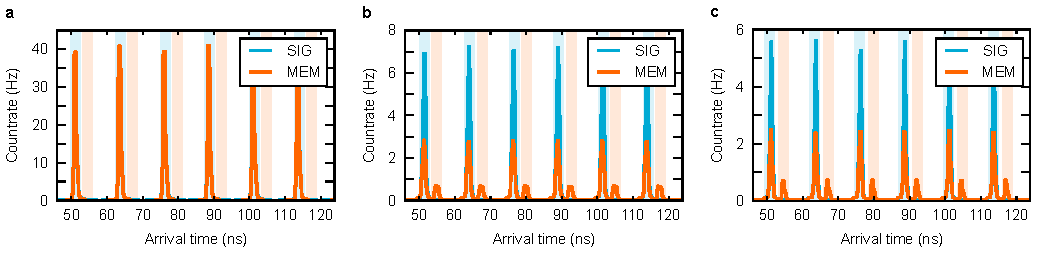
\includegraphics[width=\linewidth]{supplements_arrival_time_02.pdf}
\caption{\textbf{Sections of the arrival time histograms with indicated time gates.} \textbf{a} A section of the arrival time histogram for $\mathrm{D_{i}}$ We show the histograms for the "SIG" (blue trace) and "MEM" (orange trace) configuration. \textbf{b} A section of the arrival time histograms for detector $\mathrm{D_{s1}}$. \textbf{c} The same for detector $\mathrm{D_{s2}}$. For more details see the text.}
\label{fig:arrival_time_02}
\end{figure}

In addition to the arrival time histograms, we also recorded coincidence histograms for signal-idler two-fold coincidences ($\mathrm{D_i}$-$\mathrm{D_{s1}}$, $\mathrm{D_i}$-$\mathrm{D_{s2}}$) and the three-fold coincidences ($\mathrm{D_i}$-$\mathrm{D_{s1}}$-$\mathrm{D_{s2}}$). These are start-stop histograms, where the detection of an idler photon starts the measurement and the detection of a signal photon (the detection of a $\mathrm{D_{s1}}$-$\mathrm{D_{s2}}$ coincidence) serves as the stop signal for the two-fold (three-fold) coincidence measurement. Here, the time-bin width of the TDC was chosen to be 100~ps to ensure that the temporal resolution of the measurement was not limited by the TDC, and the time gates had a width of 3.5 ns. Again, the data was post-processed for visualization similar to the arrival time histograms. The resulting coincidence traces are plotted in Fig. \ref{fig:correlations}. Note that the unconventional shape of the traces originates from the logarithmic scaling of the y axes.

\begin{figure}
\centering
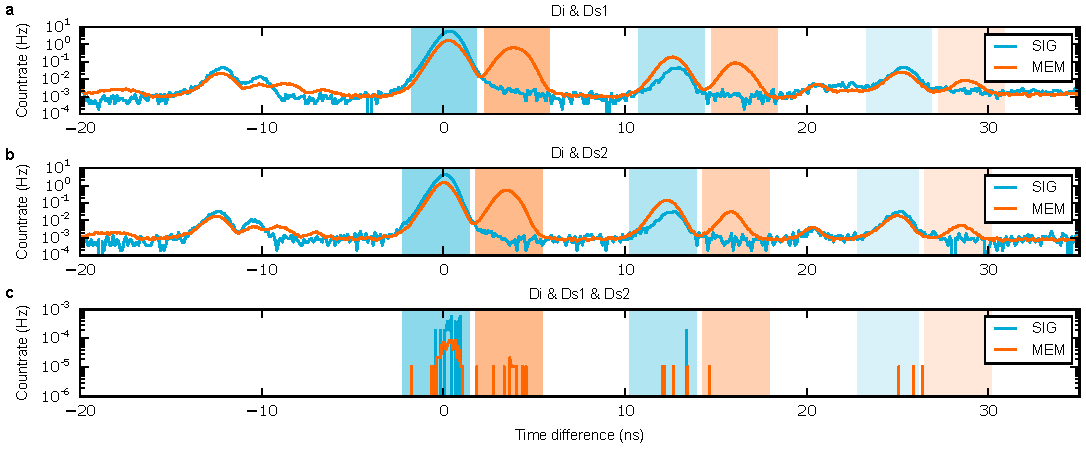
\includegraphics[width=\linewidth]{supplements_correlation.pdf}
\caption{\textbf{Correlation histograms.} \textbf{a} Accumulated normalised correlation histogram for two-fold coincidences between detectors $\mathrm{D_{i}}$ \& $\mathrm{D_{s1}}$, shown for the "SIG" (blue trace) and "MEM" (orange trace) configurations. Note the logarithmic scaling of the y axis. In the main text, we analyse the $g^{(1,1)}(0)$ cross-correlation for the initial time at 0~ns (read-in; blue-shaded) and 3.5~ns (read-out; orange-shaded). Successive read-in (read-out) time bins are indicated by shaded regions with decreasing saturation. \textbf{b} The same as in \textbf{a}, now however for two-fold coincidences between detectors $\mathrm{D_{i}}$ \& $\mathrm{D_{s2}}$. \textbf{c} Correlation histogram for three-fold coincidences between detectors $\mathrm{D_{i}}$ \& $\mathrm{D_{s1}}$ \& $\mathrm{D_{s2}}$.}
\label{fig:correlations}
\end{figure}

The "SIG" traces show a dominant peak at a time difference of 0~ns, with subsequent smaller peaks at integer multiples of the laser repetition time of 12.5~ns. From this we calculate the $g^{(1,1)}$ signal-idler cross-correlation function. The results for the "SIG" configuration are summarized in the first row of Tab. \ref{tab:g11}, where we find $g^{(1,1)}=131(1)$ for a time difference of 0~ns and $g^{(1,1)}\approx1$ for integer multiples of 12.5~ns. We also note that the values at the read-out times (3.5~ns offset from the 12.5~ns time slots) are meaningless, since there is no actual signal at the detectors. 

Turning our attention to the "MEM" configuration (orange traces in Fig. \ref{fig:correlations}), we again find a dominating peak at a time difference of 0~ns with side peaks at integer multiples of 12.5~ns. In addition, we see peaks that are offset from the major peaks by 3.5~ns. These originate from coincidence events between idler photons and signal photons that have been stored in and recalled from the memory. We also note that the side peak at 12.5~ns is higher than the corresponding peak for the "SIG" configuration. The reason for this lies in the non-unity read-out efficiency of our memory. A stored photon is not necessarily read out after 3.5~ns, but can remain stored in the memory. Then, it can be read out by the next laser pulse arriving at 12.5~ns, and so on. To quantify this effect, we again evaluate $g^{(1,1)}$. The results are summarized in the second row of Tab. \ref{tab:g11}. In this case, we find non-classical values for $g^{(1,1)}$ up to a time of 16~ns, which corresponds to around three times the lifetime of our memory. These results highlight the noise-free operation of ORCA: non-classical photon correlations are retained even after the memory efficiency has decayed to around 5\% of its initial maximum value ($1/e^3$).

\begin{table}
\centering
\begin{tabular}{|l||l|l|l|l|l|l|}
\hline
\multirow{2}{*}{}   & \multicolumn{6}{c|}{$g^{(1,1)}$} \\
%\hline
    & $\tau=0$ ns & $\tau=3.5$ ns & $\tau=12.5$ ns & $\tau=16$ ns & $\tau=25$ ns & $\tau=28.5$ ns \\
\hline\hline
SIG & 131(1) & 0.203(1) & 1.13(2) & 0.0773(1) & 1.23(2) & 0.137(1) \\
\hline
MEM & $80.5(1)$ & $120(1)$ & $9.74(2)$ & $11.3(1)$ & $1.78(2)$ & $1.19(1)$ \\
\hline
\end{tabular}
\caption{\textbf{Cross-correlation for successive read-outs.} Calculating $g^{(1,1)}$ for higher-order read-outs at integer multiples of $12.5$ ns (plus 3.5 ns for read-out pulses) yields the preservation of non-classical correlations by the memory up to around three times the memory lifetime.}
\label{tab:g11}
\end{table}

\section*{Acknowledgements}
We would like to thank R. Chrapkiewicz, M. Parniak, M. Beck, S. Gao and J. Sperling for useful discussions. We are grateful to H. Chrzanowski and P. Humphreys for proof-reading the manuscript.

This work was supported by the UK Engineering and Physical Sciences Research Council through Standard Grant No. EP/J000051/1, Programme Grant No. EP/K034480/1, and the EPSRC NQIT Quantum Technology Hub. We acknowledge support from the Air Force Office of Scientific Research: European Office of Aerospace Research and Development (AFOSR EOARD Grant No. FA8655-09-1-3020). J.N. acknowledges a Royal Society University Research Fellowship, and DJS acknowledges an EU Marie-Curie Fellowship No. PIIF-GA-2013-629229. P.M.L. acknowledges a European Union Horizon 2020 Research and Innovation Framework Programme Marie Curie individual fellowship, Grant Agreement No. 705278, and B.B. acknowledges funding from the European Union’s Horizon 2020 Research and Innovation programme under grant agreement No. 665148. I.A.W. acknowledges an ERC Advanced Grant (MOQUACINO). S.E.T. and J.H.D.M are supported by EPSRC via the Controlled Quantum Dynamics CDT under Grants EP/G037043/1 and EP/L016524/1. G.S.T. acknowledges support from the Natural Sciences and Engineering Research Council of Canada (NSERC). E.P. acknowledges an EU Marie-Curie Fellowship No. PIEF-GA-2013-627372. K.T.K. acknowledges a Santander Graduate Scholarship from Lady Margaret Hall, Oxford. O.L.-A. acknowledges Consejo Nacional de Ciencia y Tecnología (CONACyT) for support from 'Becas Conacyt Al Extranjero 2016' and Banco de M\'exico (BM) for support from 'Fondo para el Desarrollo de Recursos Humanos' (FIDERH).


\section*{Author Contributions}
K.T.K., A.F., E.P. and J.N. invented the protocol. K.T.K., G.S.T., O.L.-A., A.F. and J.N. developed the theory. K.T.K. designed the experiment. K.T.K., P.M.L., B.B., S.E.T., J.H.D.M. and D.J.S. built the setup. K.T.K. and P.M.L. conducted the experiment. B.B. wrote the data acquisition and analysis software. K.T.K., D.J.S., J.N. and I.A.W. supervised the work. All authors contributed to writing the manuscript.

\section*{Author Information} 
Reprints and permissions information is available at www.nature.com/reprints. Correspondence and requests for materials should be addressed to K.T.K. (k.kaczmarek1@physics.ox.ac.uk) or I.A.W. (i.walmsley1@physics.ox.ac.uk). K.T.K., A.F., E.P. and J.N. have jointly applied for a patent for the work presented in this paper.

\end{document}

